CORE builds on three key components---MDE, SoC, and SPL---to support large-scale model reuse. We are also interested in studying the early phases of software development, where the requirements of the software to be built are elaborated. In this chapter, we provide an overview of CORE as a reuse technique with the current state of development in Section~\ref{sec:2.1}. Then we describe UCM as part of the requirements engineering tool and its use in specifying scenarios in Section~\ref{sec:2.2}.

\section{Concern-Oriented Reuse (CORE)} \label{sec:2.1}

CORE is a reuse technique that extends MDE with best practices from advanced modularization and SoC techniques~\cite{dijkstra1976discipline}, as well as features and goal modeling to support SPL~\cite{pohl2005software}. Variations exist for any given solution 

\todo[inline]{You can reuse some of our text from previous papers here. Focus on what is really interesting for us in this thesis, i.e., interfaces, features + realization models, customization mappings, weaving algorithm. You should also show the CORE metamodel here (or at least a simplified version of it that is used as a basis for the integration in chapter 3. You can use some of the text from our SoSyM paper.}.

\subsection{Concern Interfaces}

A concern groups related models serving the same purpose, and provides three interfaces to facilitate reuse~\cite{alam2013concern}. The variation interface presents the design alternatives and their impact on non-functional requirements. The customization interface of the selected alternative details how to adapt the generic solution to a specific context. Finally, the usage interface specifies the provided behavior.

\subsubsection{Variation Interface}

\subsubsection{Customization Interface}

\subsubsection{Usage Interface}

\subsection{Reusable Aspect Models (RAM)}

\todo[inline]{No need to explain too much here, since we don't use RAM really in the rest of the thesis, no? Explain mostly that RAM is the only language currently integrated with CORE, and that the models are about design. You could use class diagrams to give an example of weaving, if you think it is necessary}.

\subsection{Customization Mappings}

\subsection{CORE Weaver}

\section{Use Case Map (UCM)} \label{sec:2.2}

\todo[inline]{Brief overview and what UCMs are used for. Maybe one example UCM (that is used later on)}.
\todo[inline]{UCM metamodel (or a simplified version of it)}.

\begin{figure}
	\centering
	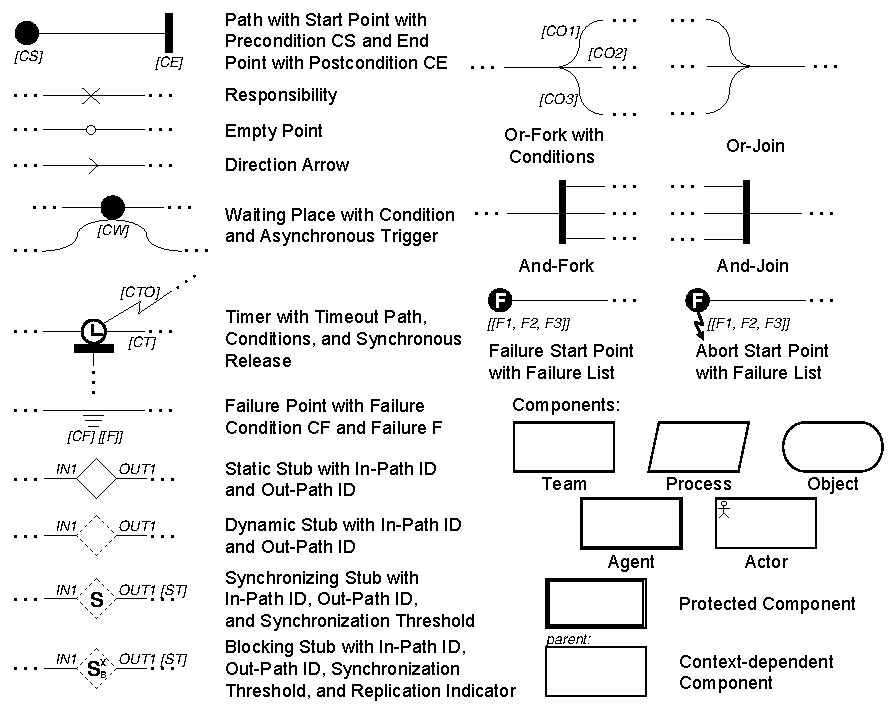
\includegraphics[scale=0.9]{fig_2_6.pdf}
	\caption[Abstract grammar: UCM metamodel]{Abstract grammar: UCM metamodel. Image courtesy of ITU~\cite{itu2012151}}
	\label{fig:2.6}
\end{figure}

\begin{figure}
	\centering
	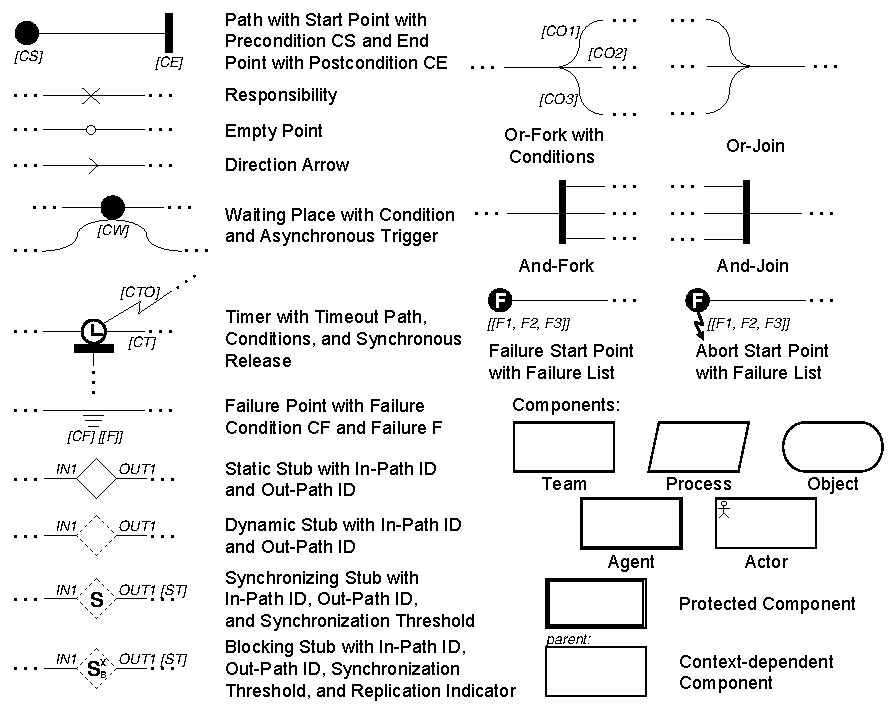
\includegraphics[scale=0.9]{fig_2_7.pdf}
	\caption[UCM notation]{UCM notation. Image courtesy of ITU~\cite{itu2012151}}
	\label{fig:2.7}
\end{figure}

\subsection{Aspect-oriented Use Case Map (AoUCM)}

\todo[inline]{Most of your related work will be Gunter's AoUCM stuff, which you probably mention above already. jUCMNav as well, but this you could also mention above when you talk about UCMs.}.
